\documentclass[]{../template/Report}%方括号内写yuxi即生成预习报告\documentclass[yuxi]{../template/Report}
\settemplatedir{../template/}%设置模板路径

\exname{弗兰克赫兹实验} %实验名称
\extable{18} %实验桌号
\instructor{韩益航} %指导教师
\class{信工2401} %班级
\name{姚舜瑜} %姓名
\stuid{3240100532} %学号

\nyear{2025} %年
\nmonth{11} %月
\nday{25} %日
\nweekday{二} %星期几，e.g. \nweekday{三}
\daypart{上午}%上午/下午

\redate{} %如有实验补做，补做日期
\resitu{} %情况说明：

\usepackage{longtable}

\begin{document}
\maketitle%输出封面

\section{预习报告（10分）}
\subsection{实验综述（5分）}
\subsubsection{实验原理}
\paragraph{波尔原子理论}

1913年，尼尔斯·波尔提出了波尔原子模型，成功解释了氢原子光谱的离散性。其基本假设包括：
\begin{enumerate}
    \item \textbf{定态假设}：原子只能处于一系列不连续的能量状态（定态），能量最低的为基态。
    \item \textbf{频率定则}：原子在能级间跃迁时吸收或辐射光子，满足 $h\nu = E_m - E_n$。
\end{enumerate}

\paragraph{弗兰克-赫兹实验原理}

本实验利用一个具有双栅结构的充氩四极电子管，即弗兰克-赫兹管，验证能级量子化。其中，本实验中原理图如\cref{yuanlitu}所示。
\begin{figure}[H]
    \centering
    
\includegraphics[width=0.5\textwidth]{yuanlitu.png}
    \caption{弗兰克-赫兹实验原理图}
    \label{yuanlitu}
\end{figure}
各电压的作用如下：
\begin{table}[H]
    \centering
    \begin{tabular}{cll}
        \hline
        符号 & 含义& 作用 \\
        \hline
        $U_{F1F2}$ & 灯丝电压&用于加热灯丝，使灯丝发出热电子 \\
        $U_{G1K}$ & 第一栅极电压&用于消除空间电荷对阴极电子发射的影响，提高发射效率。 \\
        $U_{G2K}$ & 第二栅极电压（加速电压） & 用于使从阴极K发出的电子被加速，进入管内与氩原子碰撞。 \\
        $U_{G2A}$ & 拒斥电压 & 用于筛选能量大于$eU_{G2A}$的电子到达阳极A。 \\
        $P_A$ & 微电流仪 & 用于测量通过阳极的电子电流。 \\
        $U_0$ & 第一激发电势 & 氩原子第一激发态的能量差对应的电势差。 \\
        \hline
    \end{tabular}
\end{table}

从 $0$ 开始增大 $U_{G_2K}$，会发生：
\begin{itemize}
    \item 当 $U_{G_2K} < U_0$ 时，电子能量不足以令能级跃迁，只与氩原子弹性碰撞。$U_{G_2K}$ 越大，阳极的电流就越大。
    \item 当 $U_{G_2K} = U_0$ 时，电子能量可使氩原子能级跃迁，将把全部动能传给氩原子。由于 $U_{G_2A}$ 作用，失去能量的电子不能达到阳极 $A$，电流 $I_A$ 第一次大幅度下降。
    \item 随着 $U_{G_2K}$ 继续增加，电子与原子发生非弹性碰撞的区域向 $G_1$ 移动，在 $G_2$ 附近电子重新获得的能量若小于 $U_0$，不会再发生非弹性碰撞，电子将克服 $U_{G_2A}$ 到达阳极，$I_A$ 又开始增加。
    \item 以此类推，每当 $U_{G_2K} = n U_0$ ($n=1,2,\dots$) 时，$I_A$ 都将大幅下降一次。
\end{itemize}
因此，$I_A \sim U_{G_2K}$ 曲线呈现周期性的峰谷结构（如\cref{example_figure}），峰间距即为 $U_0$。

\begin{figure}[H]
    \centering
    
\includegraphics[width=0.6\textwidth]{example_figure.png}
    \caption{弗兰克-赫兹实验典型曲线}
    \label{example_figure}
\end{figure}

\subsubsection{实验步骤}
\begin{enumerate}
    \item \textbf{测量氩原子的第一激发电势}
    
    连接实验仪与示波器。设置示波器（CH1 200mV/格, 500$\times 10^{-9}$s/格，边沿触发）。启动“自动测量”模式，观测 $I_A-U_{G_2K}$ 曲线形成。记录 7 个峰值电压，用逐差法计算 $U_0$。
    \item \textbf{测量$I_A-U_{G_2K}$曲线}
    
    切换至“手动测量”模式。缓慢调节 $U_{G_2K}$（0-100V），每隔 0.5V 记录 $I_A$，在峰谷附近加密测量。绘制曲线并计算 $U_0$。
\end{enumerate}

\subsection{实验重点（3分）}
\begin{enumerate}
    \item 验证原子能级的存在，深入理解能量“量子化”的概念。
    \item 掌握弗兰克-赫兹实验仪的使用及测量原子第一激发电势的方法。
    \item 学习处理大量实验数据，掌握利用逐差法或最小二乘法计算实验结果。
\end{enumerate}

\subsection{实验难点（2分）}
\begin{enumerate}
    \item 理解四极管中各极电压（$U_{G_1K}, U_{G_2K}, U_{G_2A}$）的作用及对实验曲线的影响。
    \item 手动测量时数据量大，需耐心操作并准确记录峰谷值附近的数据。
    \item 数据处理较为繁琐，需熟练运用软件或计算方法准确提取峰间距。
\end{enumerate}

\begin{fullreportonly}
\section{原始数据（20分）}
\begin{figure}[H]
    \centering
    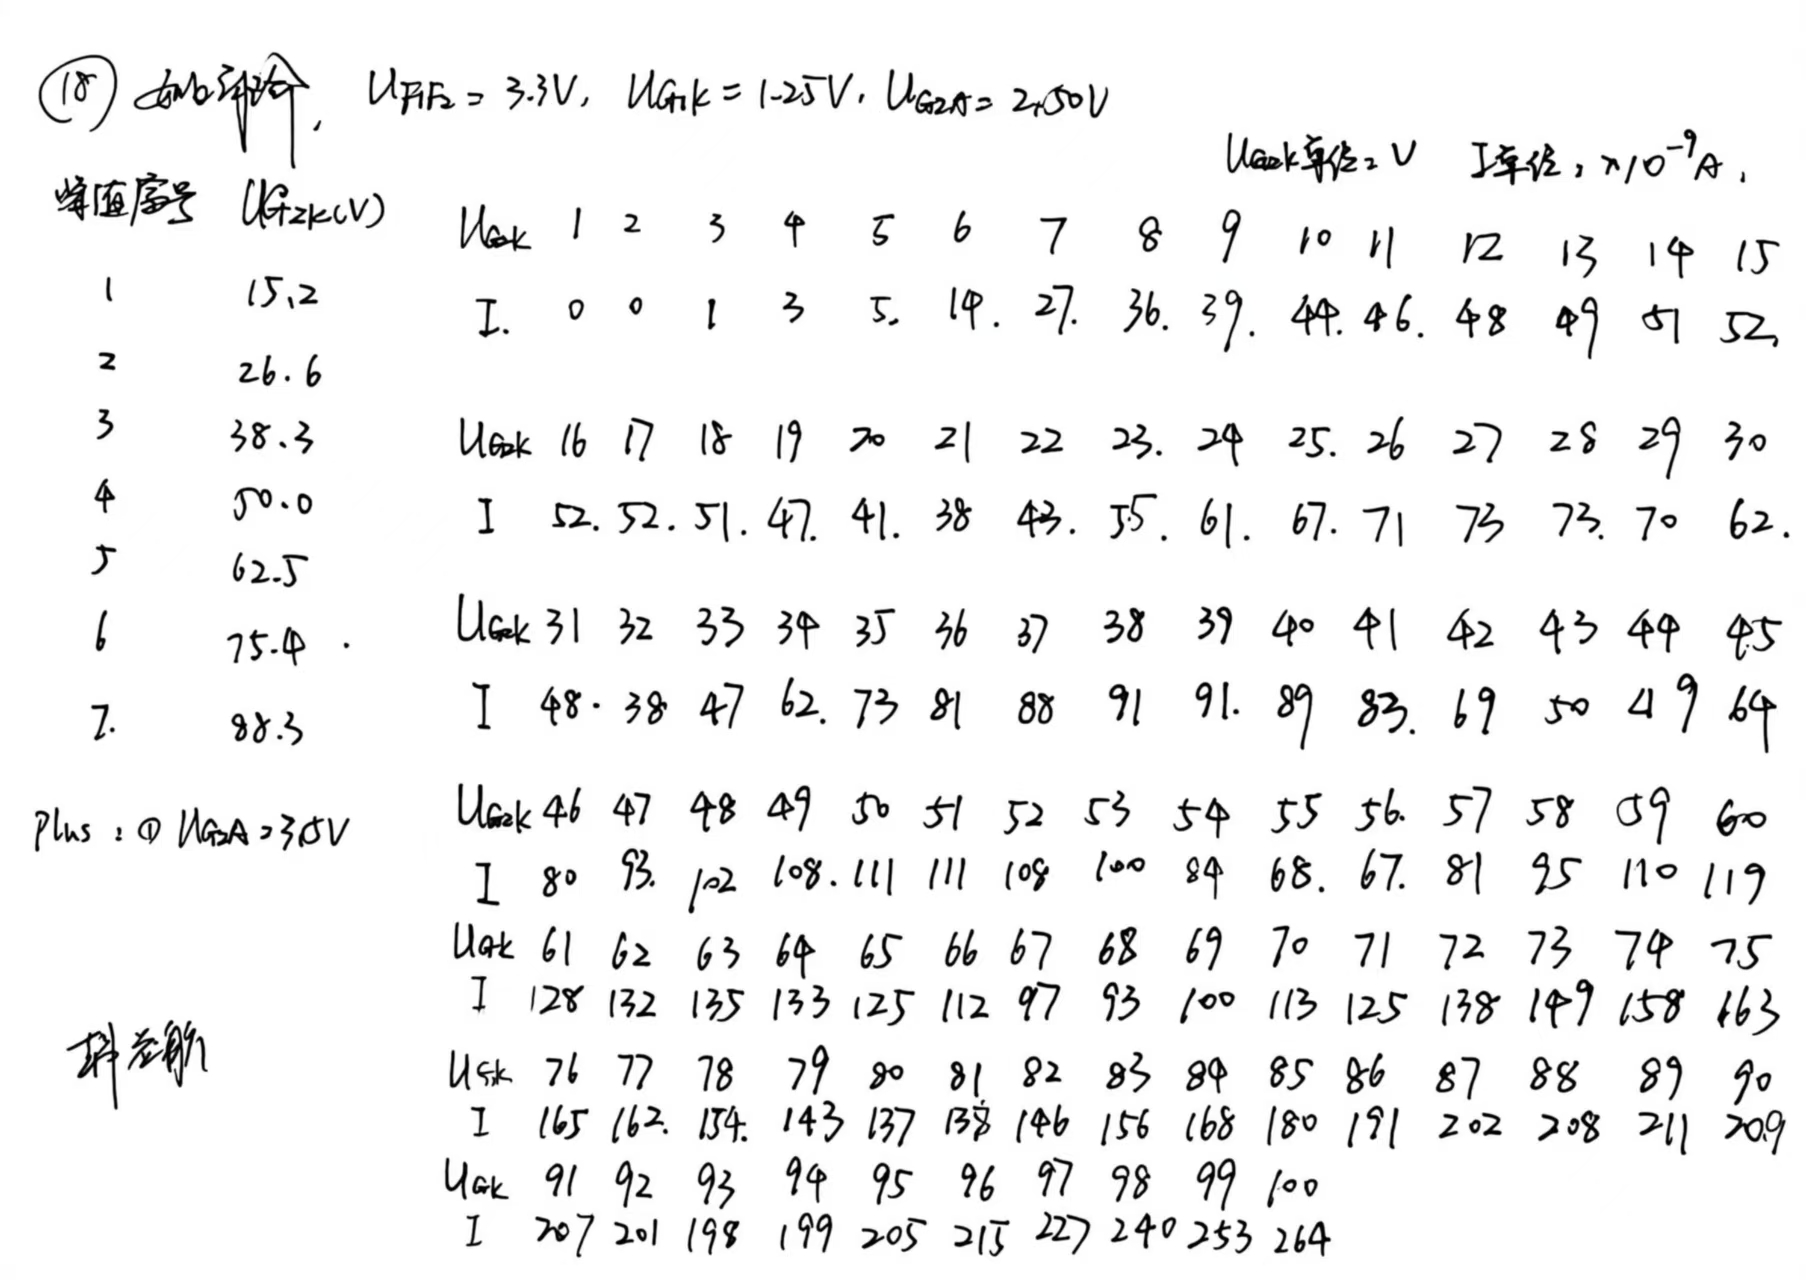
\includegraphics[width=0.55\textwidth]{figures/Y数据1.jpg}
    \caption{实验原始数据记录表}
    \label{shuju}
\end{figure}
\begin{figure}[H]
    \centering
    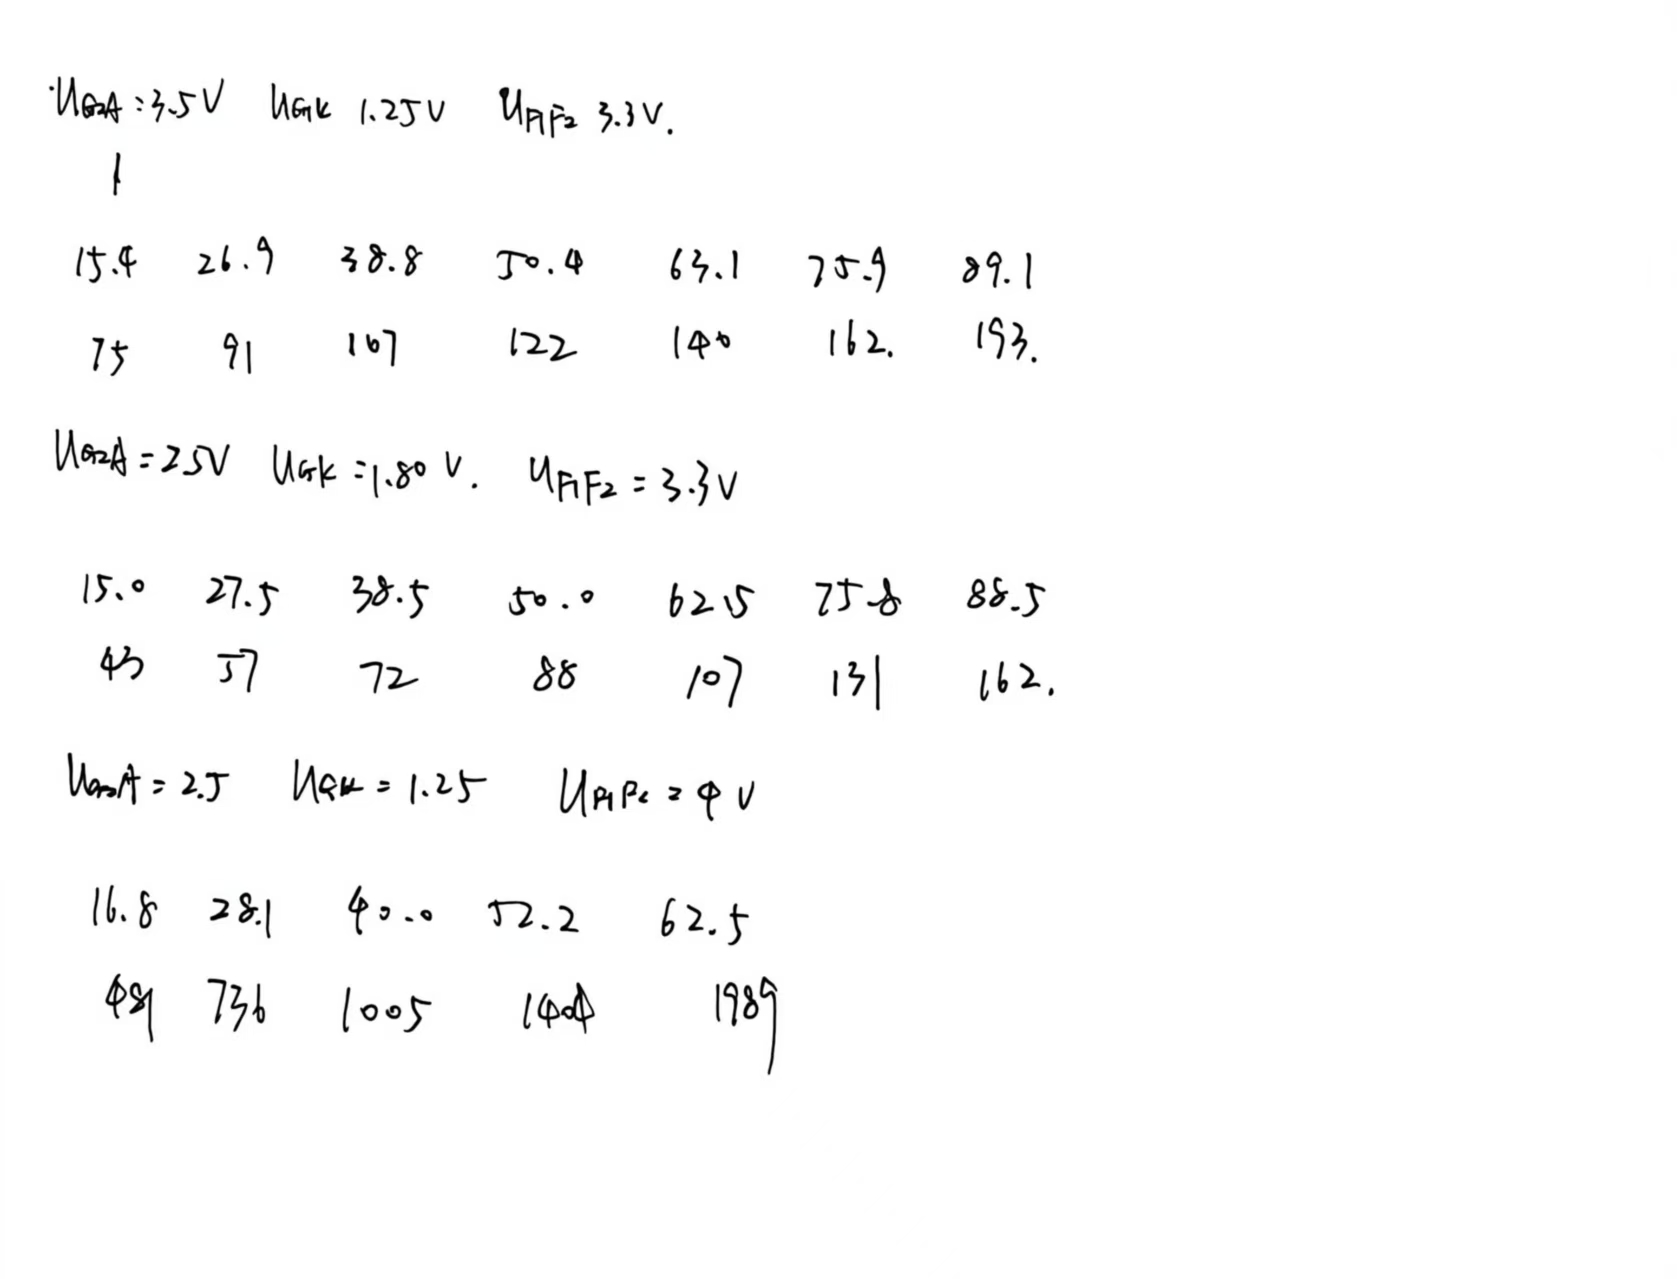
\includegraphics[width=0.55\textwidth]{figures/Y数据2.jpg}
    \caption{附加实验数据记录表}
    \label{shuju2}
\end{figure}


\section{结果与分析（60分）}
\subsection{数据处理与结果（30分）}

\subsubsection{计算氩原子第一激发电势}
通过自动测量法测量得到氩原子的各峰值电压如下表所示：
\begin{table}[H]
    \centering
    \begin{tabular}{cccccccc}
        \hline
        \multicolumn{8}{l}{条件数据：$U_{F_1F_2}=3.3V, U_{G_1K}=1.25V, U_{G_2A}=2.50V$} \\
        \hline
        峰值序号 & 1 & 2 & 3 & 4 & 5 & 6 &7\\
        \hline
        峰值电压(V) & 15.2 & 26.6 & 38.3 & 50.0 &62.5 & 75.4 & 88.3 \\
        平均峰间距 & 11.4 & 11.7 & 11.7 & 12.5 & 12.9 & 12.9 & / \\
        \hline
    \end{tabular}
    \caption{自动测量法测得的峰值电压}
    \label{tab:auto_measure}
\end{table}
由表中数据可得，氩原子第一激发电势 $U_0$ 的平均值为：
\[U_0 = \frac{11.4 + 11.7 + 11.7 + 12.5 + 12.9 + 12.9}{6} V = 12.02 V\]
利用Matlab对数据进行线性拟合，拟合结果如\cref{fig:auto_fit}所示，拟合直线斜率为 $12.18 V$，与逐差法计算结果接近。
\begin{figure}[H]
    \centering
    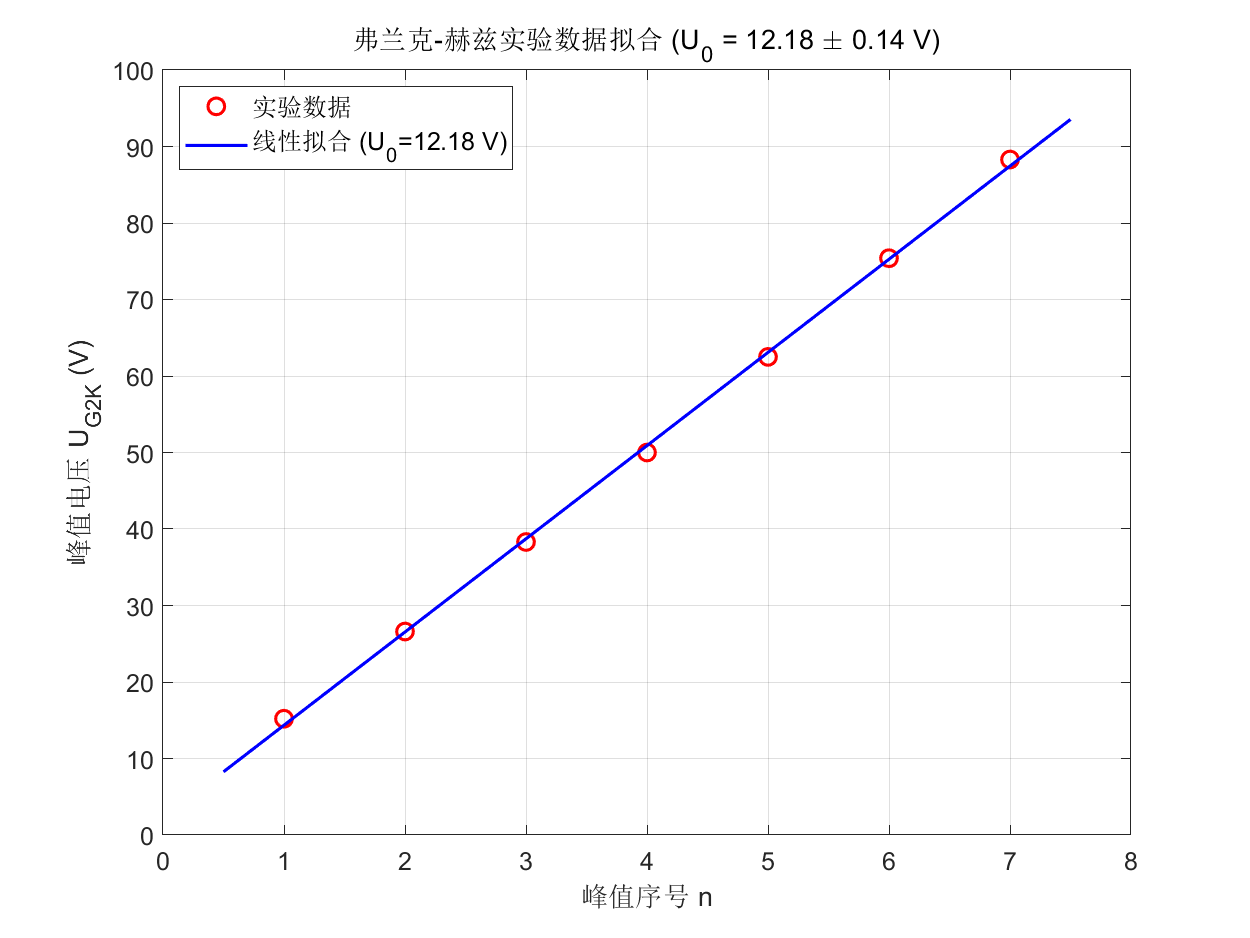
\includegraphics[width=0.55\textwidth]{figures/自动测量拟合.png}
    \caption{自动测量法数据线性拟合结果}
    \label{fig:auto_fit}
\end{figure}

\subsubsection{手动测量法测量$I_A-U_{G_2K}$曲线}
以1V为步长手动测量$I_A-U_{G_2K}$曲线，记录数据如下表所示：
\begin{longtable}{cccccccccc}
    \caption{手动测量法测得的$I_A-U_{G_2K}$数据} \label{tab:manual_measure} \\
    \hline
    $U_{G_2K}$(V) & 0.0 & 1.0 & 2.0 & 3.0 & 4.0 & 5.0 & 6.0 & 7.0 & 8.0 \\
    $I_A(\times 10^{-9} A)$ & 0.0 & 0.0 & 0.0 & 1.0 & 3.0 & 5.0 & 14.0 & 27.0 & 36.0 \\
    \hline
    $U_{G_2K}$(V) & 9.0 & 10.0 & 11.0 & 12.0 & 13.0 & 14.0 & 15.0 & 16.0 & 17.0 \\
    $I_A(\times 10^{-9} A)$ & 39.0 & 44.0 & 46.0 & 48.0 & 49.0 & 51.0 & 52.0 & 52.0 & 52.0 \\
    \hline
    $U_{G_2K}$(V) & 18.0 & 19.0 & 20.0 & 21.0 & 22.0 & 23.0 & 24.0 & 25.0 & 26.0 \\
    $I_A(\times 10^{-9} A)$ & 51.0 & 47.0 & 41.0 & 38.0 & 38.0 & 39.0 & 43.0 & 55.0 & 61.0 \\
    \hline
    $U_{G_2K}$(V) & 27.0 & 28.0 & 29.0 & 30.0 & 31.0 & 32.0 & 33.0 & 34.0 & 35.0 \\
    $I_A(\times 10^{-9} A)$ & 67.0 & 71.0 & 73.0 & 62.0 & 48.0 & 38.0 & 47.0 & 62.0 & 73.0 \\
    \hline
    $U_{G_2K}$(V) & 36.0 & 37.0 & 38.0 & 39.0 & 40.0 & 41.0 & 42.0 & 43.0 & 44.0 \\
    $I_A(\times 10^{-9} A)$ & 81.0 & 88.0 & 91.0 & 91.0 & 89.0 & 83.0 & 69.0 & 50.0 & 49.0 \\
    \hline
    $U_{G_2K}$(V) & 45.0 & 46.0 & 47.0 & 48.0 & 49.0 & 50.0 & 51.0 & 52.0 & 53.0 \\
    $I_A(\times 10^{-9} A)$ & 64.0 & 80.0 & 93.0 & 102.0 & 108.0 & 111.0 & 111.0 & 108.0 & 100.0 \\
    \hline
    $U_{G_2K}$(V) & 54.0 & 55.0 & 56.0 & 57.0 & 58.0 & 59.0 & 60.0 & 61.0 & 62.0 \\
    $I_A(\times 10^{-9} A)$ & 84.0 & 68.0 & 67.0 & 81.0 & 85.0 & 110.0 & 119.0 & 128.0 & 132.0 \\
    \hline
    $U_{G_2K}$(V) & 63.0 & 64.0 & 65.0 & 66.0 & 67.0 & 68.0 & 69.0 & 70.0 & 71.0 \\
    $I_A(\times 10^{-9} A)$ & 135.0 & 133.0 & 125.0 & 112.0 & 97.0 & 93.0 & 100.0 & 113.0 & 125.0 \\
    \hline
    $U_{G_2K}$(V) & 72.0 & 73.0 & 74.0 & 75.0 & 76.0 & 77.0 & 78.0 & 79.0 & 80.0 \\
    $I_A(\times 10^{-9} A)$ & 138.0 & 149.0 & 158.0 & 163.0 & 165.0 & 162.0 & 154.0 & 143.0 & 137.0 \\
    \hline
    $U_{G_2K}$(V) & 81.0 & 82.0 & 83.0 & 84.0 & 85.0 & 86.0 & 87.0 & 88.0 & 89.0 \\
    $I_A(\times 10^{-9} A)$ & 138.0 & 146.0 & 156.0 & 168.0 & 180.0 & 191.0 & 202.0 & 208.0 & 211.0 \\
    \hline
    $U_{G_2K}$(V) & 90.0 & 91.0 & 92.0 & 93.0 & 94.0 & 95.0 & 96.0 & 97.0 & 98.0 \\
    $I_A(\times 10^{-9} A)$ & 209.0 & 207.0 & 201.0 & 198.0 & 199.0 & 205.0 & 213.0 & 227.0 & 240.0 \\
    \hline
    $U_{G_2K}$(V) & 99.0 & 100.0&/&/&/&/&/&/\\
    $I_A(\times 10^{-9} A)$ & 253.0 & 264.0&/&/&/&/&/&/ \\
    \hline
\end{longtable}

利用Matlab对手动测量法数据进行$I_A-U_{G_2K}$曲线的绘制，结果如\cref{fig:manual_curve}所示。
\begin{figure}[H]
    \centering
    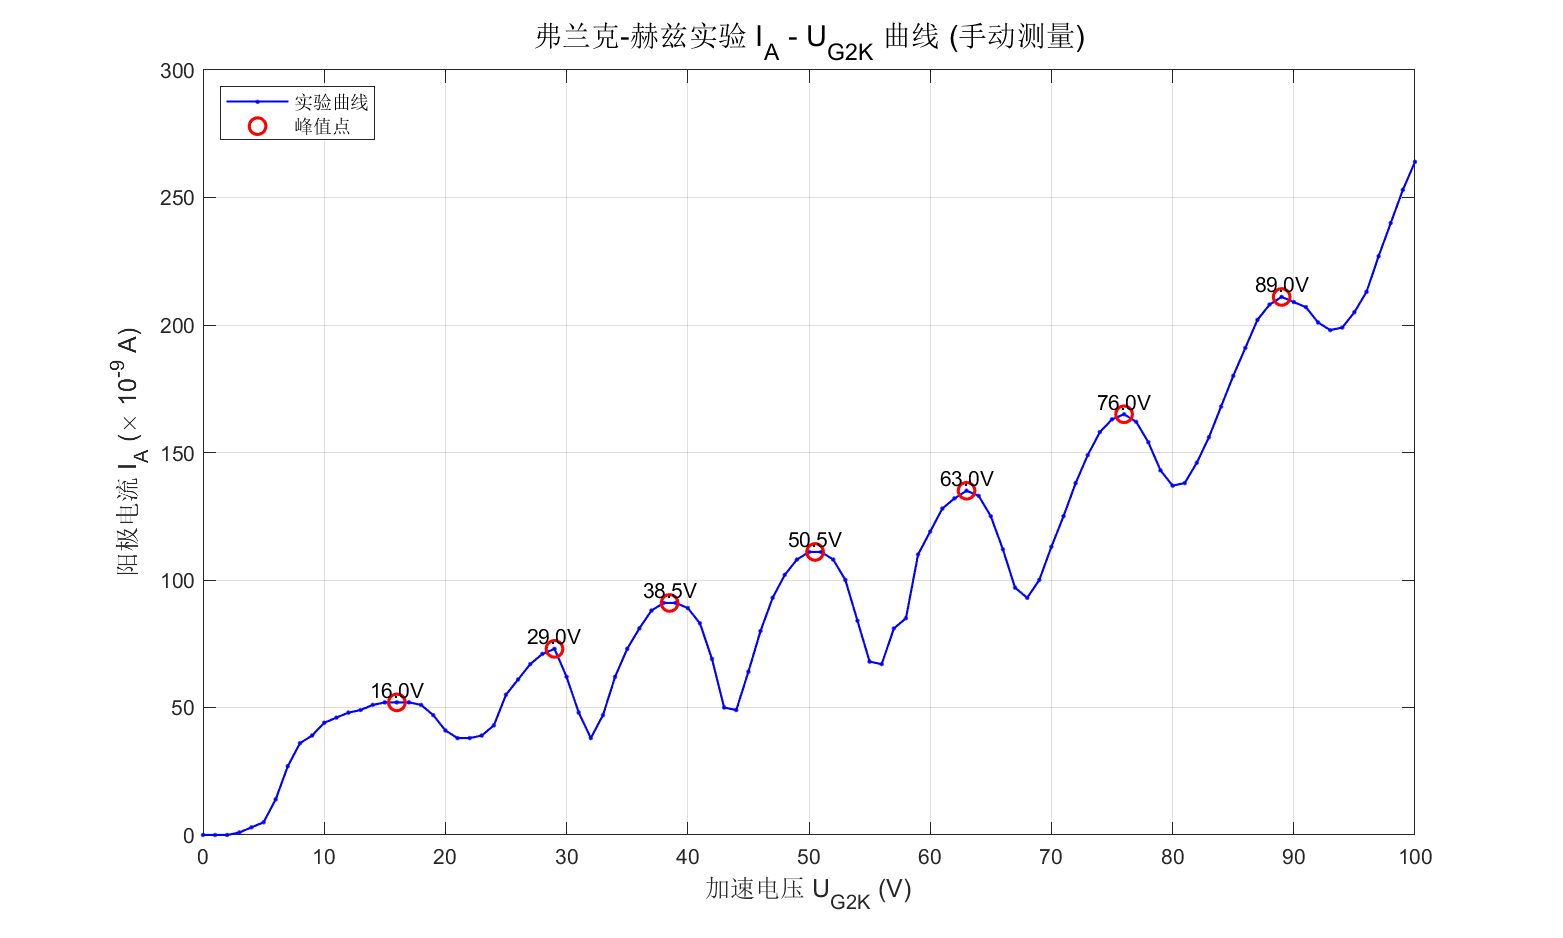
\includegraphics[width=0.65\textwidth]{figures/manual_curve.png}
    \caption{手动测量法$I_A-U_{G_2K}$曲线}
    \label{fig:manual_curve}
\end{figure}
通过观察曲线，记录7个峰值电压如下表所示：
\begin{table}[H]
    \centering
    \begin{tabular}{cccccccc}
        \hline
        峰值序号 & 1 & 2 & 3 & 4 & 5 & 6 &7\\
        \hline
        峰值电压(V) & 16.0 & 29.0 & 38.5 & 50.5 &63.0 & 76.0 & 89.0 \\
        平均峰间距 & 13.0 & 9.5 & 12.0 & 12.5 & 13.0 & 13.0 & / \\
        \hline
    \end{tabular}
    \caption{手动测量法测得的峰值电压}
    \label{tab:manual_peaks}
\end{table}
由表中数据可得，氩原子第一激发电势 $U_0$ 的平均值为：
\[U_0 = \frac{13.0 + 9.5 + 12.0 + 12.5 + 13.0 + 13.0}{6} V = 12.17 V\]
利用Matlab对数据进行线性拟合，拟合结果如\cref{fig:manual_fit}所示，拟合直线斜率为 $12.05 V$，与逐差法计算结果接近。
\begin{figure}[H]
    \centering
    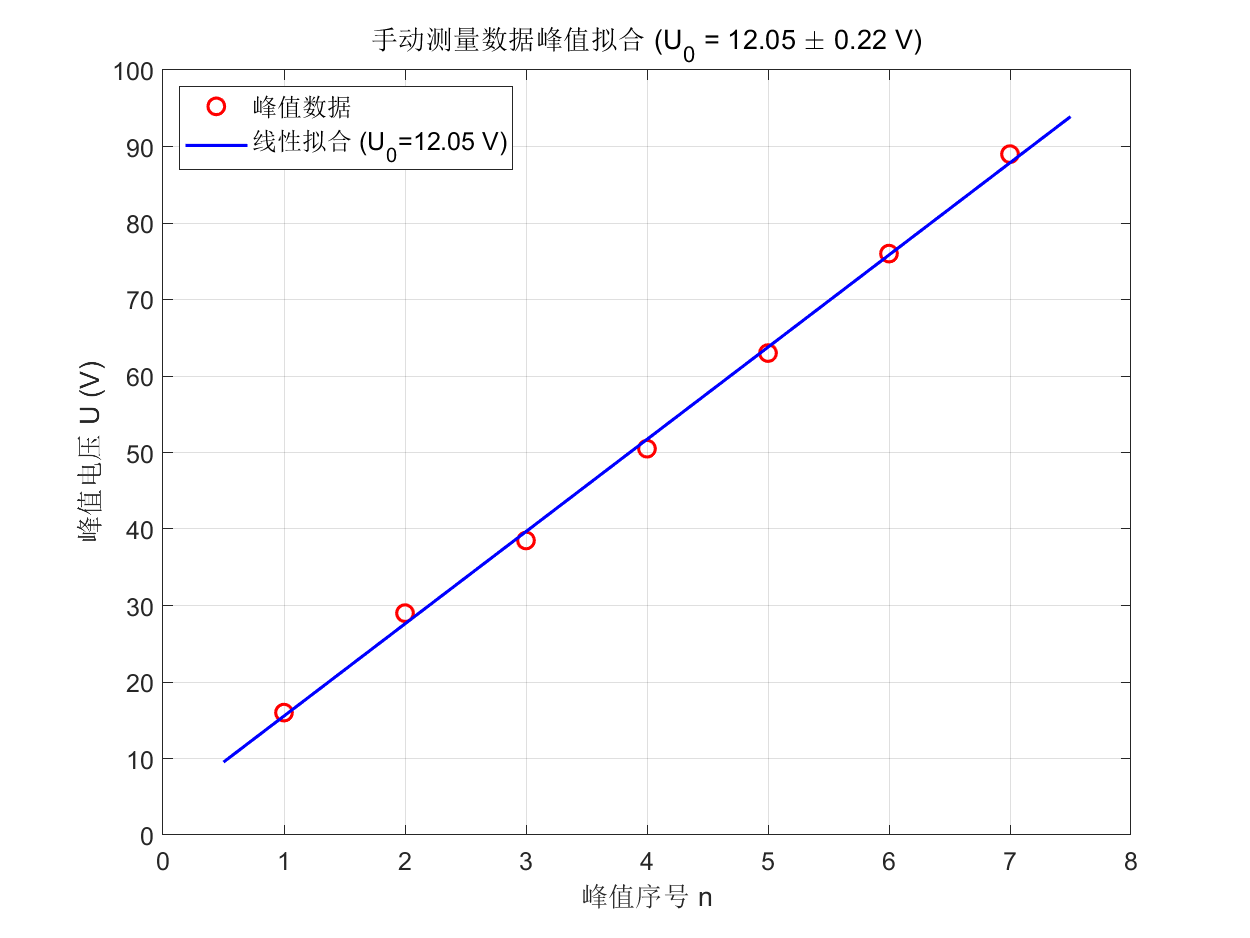
\includegraphics[width=0.6\textwidth]{figures/manual_fit.png}
    \caption{手动测量法数据线性拟合结果}
    \label{fig:manual_fit}
\end{figure}

\subsection{误差分析（20分）}
\subsubsection{氩原子第一激发电势测量实验误差}
若采取理论值 $U_0 = 11.55 V$ 作为参考，则自动测量法测得的氩原子第一激发电势相对误差为：
\[\frac{|12.18 V - 11.55 V|}{11.55 V} \approx 5.44\%\]

根据Matlab拟合结果，自动测量法测得的氩原子第一激发电势为 $U_0 = 12.18 V$，求得其斜率的A类不确定度为 $u_A = 0.1412 V$，相对不确定度为：
\[\frac{u_A}{U_0} = \frac{0.1412 V}{12.18 V} \approx 1.16\%\]

因此，自动测量法测得的氩原子第一激发电势结果为：
$$\boxed{U_0 = 12.18 V \pm 0.14 V}$$

\subsubsection{手动测量法测量实验误差}
若采取理论值 $U_0 = 11.55 V$ 作为参考，则手动测量法测得的氩原子第一激发电势相对误差为：
\[\frac{|12.05 V - 11.55 V|}{11.55 V} \approx 4.33\%\]

根据Matlab拟合结果，手动测量法测得的氩原子第一激发电势为 $U_0 = 12.05 V$，求得其斜率的A类不确定度为 $u_A = 0.2212 V$，相对不确定度为：
\[\frac{u_A}{U_0} = \frac{0.2212 V}{12.05 V} \approx 1.83\%\]

因此，手动测量法测得的氩原子第一激发电势结果为：
$$\boxed{U_0 = 12.05 V \pm 0.22 V}$$

\subsection{实验探讨（10分）}
本次实验通过自动测量法和手动测量法两种方式测量了氩原子的第一激发电势。在理论层面上，我对弗兰克赫兹实验的原理有了更深入的理解，更对量子力学中能级量子化的概念有了直观的认识。
实验过程中，我学会了如何使用弗兰克赫兹实验仪以及示波器进行数据采集和处理。自动测量法提高了数据采集的效率，而手动测量法则让我更加细致地观察了$I_A-U_{G_2K}$曲线的变化。
在数据处理方面，我掌握了逐差法和线性拟合法来计算氩原子第一激发电势，并通过误差分析了解了实验结果的准确性和可靠性。

\subsection{附加实验}
附加实验将探讨$U_{G_1K}, U_{G_2K}, U_{G_2A}$对$I_A-U_{G_2K}$曲线的影响。通过改变各电压参数，观察曲线变化规律，并通过自动测量记录数据进行定性分析.




\subsubsection{初始条件下的曲线}
其中，初始条件为$U_{F_1F_2}=3.3V, U_{G_2A}=2.50V, U_{G_1K}=1.25V$。
初始条件的$I_A-U_{G_2K}$曲线如\cref{fig:initial_curve}所示。
\begin{figure}[H]
    \centering
    \includegraphics[width=0.6\textwidth]{figures/新建文件1.png}
    \caption{初始条件下的$I_A-U_{G_2K}$曲线}
    \label{fig:initial_curve}
\end{figure}









\subsubsection{$U_{G_1K}$对$I_A-U_{G_2K}$曲线的影响}
$U_{G1K}$是一个预加速电压，用于将电子从阴极拉出并穿过第一栅极G1,与拒斥电压$U_{G2A}$共同构成了一个筛选电子的“能量门槛”。
\par
若增大$U_{G1K}$，电子在进入主加速区（G1-G2）之前就获得了较高的初始能量，使得电子只需一个较小的$U_{G2K}$就能达到激发氩原子的临界能量$U_0$。因此，曲线的第一个峰值位置会向左移动。同时，更多的低能电子因此有足够能量到达板极，曲线起始段的电流会更大。
反之，减小$U_{G1K}$会使第一个峰值位置向右移动。
\par
一旦电子开始周期性获得并损失能量，后续峰谷的间距依然是原子的本征属性，基本不变。但需要注意的是，$U_{G1K}$设置不当可能导致曲线起始段畸变，影响第一个$U_0$值的准确读取。

保持$U_{F_1F_2}=3.3V, U_{G_2A}=2.50V$，设置$U_{G_1K}=1.80V$，测量$I_A-U_{G_2K}$曲线，示波器结果如\cref{fig:UG1K_effect}所示。
\begin{figure}[H]
    \centering
    \includegraphics[width=0.5\textwidth]{figures/新建文件2.png}
    \caption{$U_{G_1K}$对$I_A-U_{G_2K}$曲线的影响}
    \label{fig:UG1K_effect}
\end{figure}
用自动法测得各个峰值电压如下表所示：
\begin{table}[H]
    \centering
    \begin{tabular}{cccccccc}
        \hline
        \multicolumn{8}{l}{条件数据：$U_{F_1F_2}=3.3V, U_{G_2A}=2.50V, U_{G_1K}=1.80V$} \\
        \hline
        峰值序号 & 1 & 2 & 3 & 4 & 5 & 6 &7\\
        \hline
        峰值电压(V) & 15.0 & 27.5 & 38.5 & 50.0 &62.5 & 75.6 & 88.5 \\
        平均峰间距 & 12.5 & 11.0 & 11.5 & 12.5 & 13.1 & 12.9 & / \\
        对应电流(nA) & 43 & 57 & 72 & 88 & 107 & 131 & 162 \\
        \hline
    \end{tabular}
    \caption{自动测量法测得的峰值电压（$U_{G_1K}=1.80V$）}
    \label{tab:UG1K_peaks}
\end{table}








\subsubsection{$U_{G_2A}$对$I_A-U_{G_2K}$曲线的影响}
$U_{G2A}$在第二栅极G2和板极A之间建立一个反向的减速电场,只有碰撞后剩余动能大于$eU_{G2A}$的电子才能克服该电场到达板极形成电流$I_A$。
\par
增大$U_{G2A}$会提高电子到达板极的能量门槛。在峰值处，电子刚刚经历非弹性碰撞，能量损失最大，本已勉强能越过门槛，现在门槛提高，它们更难以到达板极，导致峰值电流显著下降。而在谷值处，电子因能量不足无法激发原子，本身剩余能量就高，门槛提高对它们的影响相对较小。
综合效果就是，峰谷差值变小，曲线变得平坦，峰谷对比度下降，同时整体电流水平降低。
\par
同理，减小$U_{G2A}$会降低电子到达板极的门槛，使得峰值电流增加，峰谷差值增大，曲线峰形更尖锐。
\par
理论上，峰位由碰撞能量决定，与筛选条件无关，因此$U_0$不变，但在实际测量中，如果$U_{G2A}$过大，会导致峰值过于平坦而难以精确判定其位置，引入测量误差。

保持$U_{G_1K}=1.25V, U_{F_1F_2}=3.3V$，设置$U_{G_2A}=3.5V$，测量$I_A-U_{G_2K}$曲线，示波器结果如\cref{fig:UF1F2_effect}所示。
\begin{figure}[H]
    \centering
    \includegraphics[width=0.48\textwidth]{figures/新建文件3.png}
    \caption{$U_{G_2A}$对$I_A-U_{G_2K}$曲线的影响}
    \label{fig:UF1F2_effect}
\end{figure}
用自动法测得各个峰值电压如下表所示：
\begin{table}[H]
    \centering
    \begin{tabular}{cccccccc}
        \hline
        \multicolumn{8}{l}{条件数据：$U_{F_1F_2}=3.3V, U_{G_1K}=1.25V, U_{G_2A}=3.5V$} \\
        \hline
        峰值序号 & 1 & 2 & 3 & 4 & 5 & 6 &7\\
        \hline
        峰值电压(V) & 15.4 & 26.9 & 38.8 & 50.4 &63.1 & 75.9 & 89.1 \\
        平均峰间距 & 11.5 & 11.9 & 11.6 & 12.7 & 12.8 & 13.2 & / \\
        对应电流(nA) & 75 & 91 & 107 & 122 & 140 & 162 & 193 \\
        \hline
    \end{tabular}
    \caption{自动测量法测得的峰值电压（$U_{G_2A}=3.5V$）}
    \label{tab:UG2A_peaks}
\end{table}











\subsubsection{$U_{F_1F_2}$对$I_A-U_{G_2K}$曲线的影响}
灯丝电压决定了阴极的加热温度，进而决定了单位时间内发射出的热电子数量（即发射电流），主要影响曲线的整体幅度，而非峰值位置。
\par
当增大$U_{F1F2}$时，阴极温度升高，发射的电子流密度显著增加，导致$I_A$整体增大，曲线的峰值和谷值均上移，但峰间电压间隔保持不变。
\par
同理，减小$U_{F1F2}$会导致曲线整体下移，但即第一激发电位$U_0$的测量值基本不变。

保持$U_{G_2A}=2.5V, U_{G_1K}=1.25V$，设置$U_{F_1F_2}=4.00V$，测量$I_A-U_{G_2K}$曲线，示波器结果如\cref{fig:UG2A_effect}所示。
\begin{figure}[H]
    \centering
    \includegraphics[width=0.49\textwidth]{figures/新建文件4.png}
    \caption{$U_{F_1F_2}$对$I_A-U_{G_2K}$曲线的影响}
    \label{fig:UG2A_effect}
\end{figure}
用自动法测得各个峰值电压如下表所示：
\begin{table}[H]
    \centering
    \begin{tabular}{cccccc}
        \hline
        \multicolumn{6}{l}{条件数据：$U_{F_1F_2}=4.0V, U_{G_1K}=1.25V, U_{G_2A}=2.50V$} \\
        \hline
        峰值序号 & 1 & 2 & 3 & 4 & 5\\
        \hline
        峰值电压(V) & 16.8 & 28.1 & 40.0 & 52.2 & 62.5 \\
        平均峰间距 & 11.3 & 11.9 & 12.2 & 10.3 & / \\
        对应电流(nA) & 481 & 736 & 1005 & 1404 & 1989 \\
        \hline
    \end{tabular}
    \caption{自动测量法测得的峰值电压（$U_{F_1F_2}=4.0V$）}
    \label{tab:UF1F2_peaks}
\end{table}




\section{思考题（10分）}
\subsection{第一激发电位的物理含义是什么?}
\paragraph{答：}
第一激发电位是原子从基态跃迁到第一激发态所需要的最小能量对应的电势差。它反映了原子内部能级的离散性，即能量量子化。在本实验中，当电子获得的动能达到氩原子的第一激发电位对应的能量时，电子与氩原子发生非弹性碰撞，将能量传递给氩原子使其跃迁，电子自身失去能量。

\subsection{温度对$F-H$管的$I_A-U_{G2K}$曲线的影响有哪些?}
\paragraph{答：}
温度主要通过影响灯丝发射电子的能力和管内气体原子的热运动来影响曲线：
\begin{enumerate}
    \item \textbf{影响热电子发射}：温度升高，会使阴极发射的热电子数量显著增加，导致阳极电流 $I_A$ 整体大幅增大。
    \item \textbf{影响平均自由程}：温度变化会改变管内气体的压强和密度，从而影响电子的平均自由程。若温度过高，碰撞过于频繁，电子难以积累足够能量；若温度过低，碰撞概率降低，现象不明显。
\end{enumerate}
\end{fullreportonly}
\insertnotes
\end{document}



第一组数据 (参数: V_{G2A}=3.5V, V_{G1K}=1.25V, V_{F1F2}=3.3V)

峰值序号	峰值电压 (V)	信号 (I)
1	15.4	75
2	26.9	91
3	38.8	107
4	50.4	122
5	63.1	140
6	75.9	162
7	89.1	193

第二组数据 (参数: V_{G2A}=2.5V, V_{G1K}=1.80V, V_{F1F2}=3.3V)

峰值序号	峰值电压 (V)	信号 (I)
1	15.0	43
2	27.5	57
3	38.5	72
4	50.0	88
5	62.5	107
6	75.6	131
7	88.5	162

第三组数据 (参数: V_{G2A}=2.5V, V_{G1K}=1.25V, V_{F1F2}=4V)

峰值序号	峰值电压 (V)	信号 (I)
1	16.8	481
2   28.1    736
3	40.0    1005
4	52.2    1404
5   62.5   1989